\documentclass[a4paper]{article}
\usepackage[utf8]{inputenc}
\usepackage[russian,english]{babel}
\usepackage[T2A]{fontenc}
\usepackage[left=10mm, top=20mm, right=18mm, bottom=15mm, footskip=10mm]{geometry}
\usepackage{indentfirst}
\usepackage{amsmath,amssymb}
\usepackage[italicdiff]{physics}
\usepackage{graphicx}
\usepackage{multirow}
\usepackage{svg}
\graphicspath{{images/}}
\DeclareGraphicsExtensions{.pdf,.png,.jpg}
\usepackage{wrapfig}
\usepackage{caption}
\captionsetup[figure]{name=Рисунок}
\captionsetup[table]{name=Таблица}
\title{\underline{Изучение плазмы газового разряда в неоне}}
\author{Каспаров Николай, Б01-304}

\begin{document}

\maketitle
\begin{center}
\Large{\textbf{ }}
\end{center}

\subparagraph{Цель работы:}

\begin{itemize}
\item Изучение вольт-амперной характеристики тлеющего разряда;
\item Изучение свойств плазмы методом зондовых характеристик.
\end{itemize}

\subparagraph{В работе используются:}

\begin{itemize}
\item Стеклянная газоразрядная трубка, наполненная неоном;
\item Высоковольтный источник питания (ВИП);
\item Источник питания постоянного тока;
\item Делитель напряжения;
\item Потенциометр, амперметры, вольтметры, переключатели.
\end{itemize}

\section{Теоретическое введение}

\subsection{Плазменная частота}

Выделим в нейтральной плазме некоторый объём в виде параллелепипеда (см. рис. 1).

\begin{wrapfigure}{l}{0.4\textwidth}
    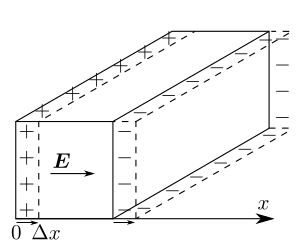
\includegraphics[width = 0.35\textwidth]{freq.png}
    \caption[width = 0.95\textwidth]{Плазменные колебания}
\end{wrapfigure}

Обозначим концентрацию электронов как $n_e$, однозарядных ионов: $n_i$, тогда $n_i=n_e$.
Пусть все электроны сместились на расстояние $x$ относительно ионов.
Будем считать, что ионы неподвижны,
тогда на боковых гранях параллелепипеда возникнут нескомпенсированные поверхностные заряды с плотностью

\begin{equation}
    \sigma = \pm n_e e \Delta x.
\end{equation}

Аналогично конденсатору, они создадут электрическое поле
\begin{equation}
    E = 4 \pi n_e e \Delta x.
\end{equation}

В свою очередь это поле будет действовать на электроны:
\begin{equation}
    \frac{d^2 \Delta x}{dt^2} = - \frac{eE}{m} = - \frac{4 \pi n_e e^2}{m} \Delta x.
\end{equation}
Видно, что полученное уравнение описывает гармонические колебания с частотой
\begin{equation}
    w_p = \sqrt{\frac{4 \pi n_e e^2}{m_e}}
\end{equation}

Таким образом, мы получили частоту коллективных колебаний электронов относительно квазинейтрального состояния. Такие колебания на­
зывают ленгмюровскими, а частоту $\omega_p$ — плазменной или ленгмюровской.

\subsection{Плазменная частота}
Плазменные колебания могут быть возбуждены как за счёт внешнего воздействия
(например, при прохождении электромагнитной волны),
так и за счёт тепловой энергии, содержащейся непосредственно в плазме.
Оценим амплитуду колебаний в последнем случае.

Средняя скорость теплового движения электронов по порядку величины равна
\begin{equation}
    v_e \sim \sqrt{\frac{kT_e}{m_e}}.
\end{equation}
Амплитуду $r$ колебаний электронов относительно ионов можно оценить как
смещение с тепловой скоростью $\overline{v_e}$ за характерное время плазменных колбений 
$1/\omega_p$. Полученную величину обозначают как 
\begin{equation}
    r_D = \sqrt{\frac{kT_e}{4 \pi n_e e^2}} \sim \frac{\overline{v_e}}{\omega_p}
\end{equation}
и называют дебаевским радиусом (или дебаевской длиной).
Это — ещё один важный плазменный параметр, задающий характерный
пространственный масштаб многих плазменных явлений.

\subsection{Измерения методом одиночного зонда}

При внесении проводника в плазму, он подвергается «бомбардировке» со стороны её заряженных частиц.
Как известно из молекулярной физики, число частиц,
ударяющихся в идеальном газе в секунду о единичную поверхность, равно:

\begin{equation}
    j = \frac{1}{4} n \overline{v},
\end{equation}
и так как скорость электронов, очевидно, больше скоростей ионов, проводник зарядится отрицательно.

Найдем отрицательный потенциал $U_f$ (относительно плазмы), который также называется плавающим.
В равновесии, если бы $U_f = 0$, то электронный и ионные токи было бы равны:
\begin{equation}
    I_{e0} = \frac{n \overline{v}_e}{4}eS, \qquad I_{i0} = \frac{n \overline{v}_i}{4}eS,
\end{equation}

Теперь учтем, что $U_f \neq 0$. На ионный ток это почти не повлияет: $I_i \approx I_{i0}$.
Электронный же ток уменьшится, посколько лишь часть электронов, летящих к зонду,
способна преодолеть потенциальный барьер. Из распределения Больцмана:

\begin{equation}
    I_e = I_{e0} \exp(\frac{eU_f}{kT_e}), 
\end{equation}
где $U_f < 0$, поэтому $I_e < I_{e0}$.

\begin{wrapfigure}{l}{0.4\textwidth}
    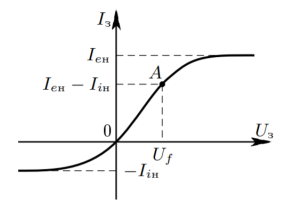
\includegraphics[width = 0.35\textwidth]{bomon.png}
    \caption[width = 0.95\textwidth]{Ток насы}
\end{wrapfigure}

Будем подавать потенциал $U_\text{з}$ на зонд и снимать значение
зондового тока $I_\text{з}$. Максимальное значение тока $I_\text{eн}$ – электронный ток насыщения,
а минимальное $I_\text{iн}$ – ионный ток насыщения.
Значение из эмпирической формулы Бомона:

\begin{equation}
    I_\text{iн} = 0.4neS \sqrt{\frac{2kT_e}{m_i}}
\end{equation}

\subsection{Измерения методом двойного зонда}
Двойным зондом называется система, состоящая из двух одинаковых зондов,
расположенных на небольшом расстоянии друг от друга.
Между зондами создаётся разность потенциалов $U$, которая по величине
много меньше плавающего потенциала $|U| \ll |U_f|$.

При небольших разностях потенциалов ионные
токи на оба зонда близки к току насыщения и компенсируют друг друга, а значит величина
результирующего тока полностью связана с разностью электронных токов. Пусть потенциалы на зондах равны:

\begin{equation}
    U_1 = U_f + \Delta U_1, \qquad U_2 = U_f + \Delta U_2,
\end{equation}
где $\Delta U_1, \Delta U_2 \ll U_f$. Напряжение между зондами равно

\begin{equation}
    U = U_2 - U_1 = \Delta U_2 - \Delta U_1.
\end{equation}

Найдем ток, приходящий на первый электрод:

\begin{equation}
    I_1 = I_\text{iн} - I_\text{e0} \exp(\frac{eU_1}{kT_e}) = I_\text{iн} - \left[ I_\text{e0} \exp(\frac{eU_f}{kT_e}) \right] \exp(\frac{e \Delta U_1}{kT_e}),
\end{equation}
но заметим, что при $\Delta U_1 = 0$ ($U_1 = U_f$) электронный и ионный токи компенсируют друг друга.
Значит, 
\begin{equation}
    I_1 = I_\text{iн} - I_\text{e0} \exp(\frac{e \Delta U_1}{kT_e}),
\end{equation}
\begin{equation}
    I_2 = I_\text{iн} - I_\text{e0} \exp(\frac{e \Delta U_2}{kT_e}),
\end{equation}

Из последовательности соединения видно, что $I_1 = -I_2 = I$, значит

\begin{equation}
    U = \Delta U_1 - \Delta U_2 = \frac{kT_e}{e} \ln \frac{I_\text{iн} - I}{I_\text{iн} + I},
\end{equation}

и, разрешая это равенство относительно $I$, получаем:

\begin{equation}
    I = I_\text{iн} \th \frac{eU}{2kT_e}.
\end{equation}

Отсюда, используя приближение $\th x \approx x$, получим
\begin{equation}
    kT_e = \frac{1}{2} \frac{eI_\text{iн}}{\frac{dI}{dU}|_{U = 0}},
\end{equation}
где $\frac{dI}{dU}|_{U = 0}$ - наклон характеристики зонда вблизи начала координат.

В действительности же, наш результат отличается от реального существованием наклона у асимптот в области больших $|U|$,
что связано с ускорением частиц плазмы приложенным полем, которое не учтено при выводе

\begin{figure}[h!]
    \centering
    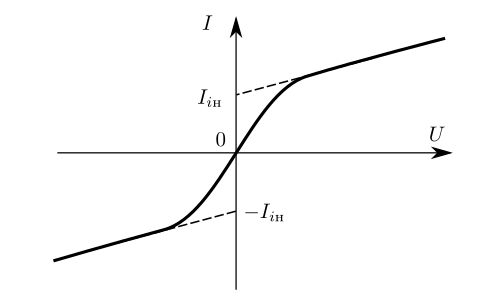
\includegraphics[width=0.5\pdfpagewidth]{VAH.png}
    \caption{ВАХ двойного зонда}
\end{figure}

\newpage

\section{Описание установки}

\begin{figure}[h!]
    \centering
    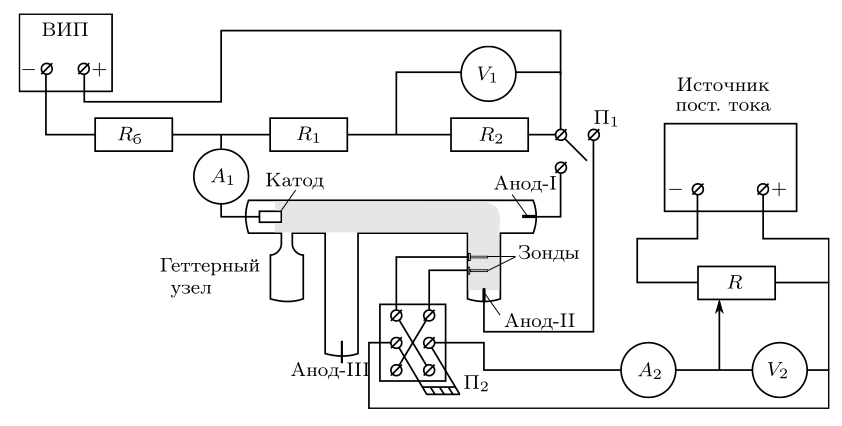
\includegraphics[width=0.8\pdfpagewidth]{scheme.png}
    \caption{Схема установки}
\end{figure}

Стеклянная газоразрядная трубка имеет холодный (ненакаливаемый) полый катод, три анода и \textit{геттерный} узел -- стеклянный баллон, на внутреннюю повехность которого напылена газопоглощающая плёнка (\textit{геттер}). Трубка наполнена изотопом неона $^{22}$Ne при давлении 2 мм рт. ст. Катод и один из анодом (I и II) с помощью переключателя $\Pi_1$ подключается через балластный резистор $R_\text{б}$ ($\approx 450$ кОм) к регулируемому ВИП с выкодным напряжением до 4 кВ.\\
При подключении к ВИП анода-I между ним и катодом возникает газовый разряд. Ток разряда измеряется миллиамперметром $A_1$, а падение напряжения на разрядной трубке -- цифровым вольтметром $V_1$, подключённым к трубке черезе высокоомный (25 МОм) делитель напряжения с коэффициентом $(R_1+R_2)/R_2 = 10$.\\
При подключении к ВИП анода-II разряд возникает в пространстве между катодом и анодом-II, где находятся двойной зонд, используемый для диагностики плазмы положительного столба. Зонды изготовлены из молибденовой проволоки диаметром $d = 0.2$ мм и имеют длину $l = 5.2$ мм. Они подключены к источнику питания GPS через потенциометр $R$. Переключатель $\Pi_2$ позволяет изменять полярность напряжения на зондах. Величина напряжения на зондах изменяеься с помощью дискретного переключателя <<$V$>> выходного напряжения источника питания и потенциометра $R$, а измеряется цифровым вольтметром $V_2$. Для измерения зондового тока используется мультиметр $A_2$.

\newpage

\section{Ход работы}

\subsection{Вольт-амперная характеристика разряда}

\begin{wrapfigure}{l}{0.50\textwidth}
    \vspace{-0.7cm}
    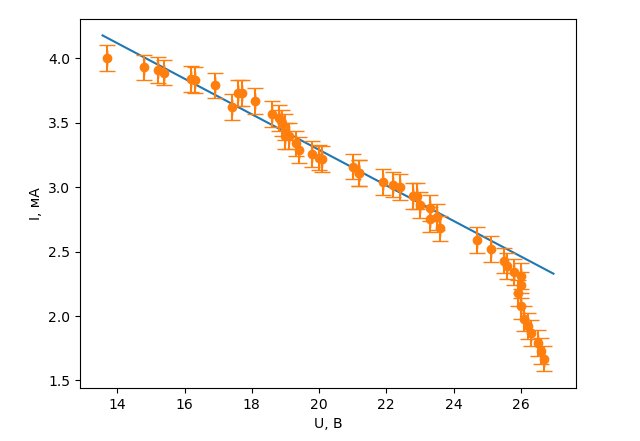
\includegraphics[width = 0.50\textwidth]{VAH_1.png}
    \caption[width = 0.50\textwidth]{ВАХ разряда}
\end{wrapfigure}

\vspace{0.5cm}

Будем увеличивать напряжение ВИП, пока не произойдет зажигание разряда.
Затем обратно, до исчезновения разряда. Данные нанесем на график (Рис. 5):

Разницы в результатах при повышении и понижении напряжения обнаружено не было.
Аппроксимируем график прямой (используя МНК).\\
Найдем дидифференциальное сопротивление разряда:

\begin{equation}
    R_\text{диф} = \frac{dU}{dI} = (-7.0 \pm 0.2) \ \text{кОм}
\end{equation}


\\\
\\\
\\\
\\\
\\\
\\\

Как мы может увидеть из Рис. 6, участок разряда в нашем случае соответсвует 
фрагменту ДГ - поднормальному тлеющему разряду.
\begin{figure}[h!]
    \centering
    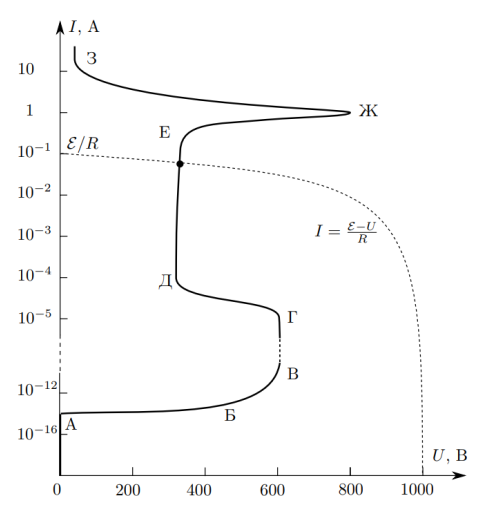
\includegraphics[width = 0.50\textwidth]{VAH_REF.png}
    \caption[width = 0.50\textwidth]{ВАХ разряда}
\end{figure}

\newpage

\subsection{Зондовые характеристики}

Снимем ВАХ двойного зонда для токов разряда 2 мА, 3 мА и 4 мА.
Каждый график отцентрируем и нанесем на общую систему координат:

\begin{figure}[h!]
    \centering
    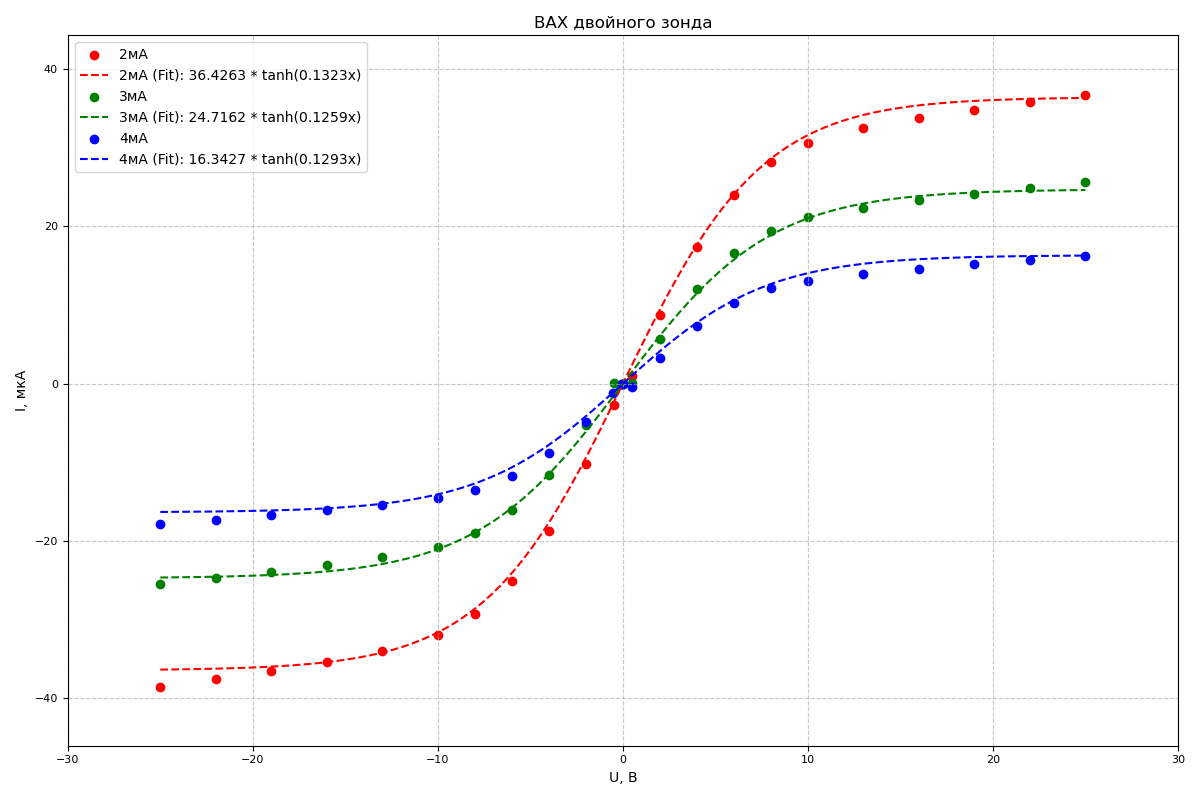
\includegraphics[width=0.8\pdfpagewidth]{VAH_2.png}
    \caption{ВАХ двойного зонда}
\end{figure}

Вспомним формулу (17):

\begin{equation*}
    I = I_\text{iн} \th \frac{eU}{2kT_e}.
\end{equation*}

Из графика получим ионный ток насыщения для разных сил тока, а также температуру электронов $T_e$.
Используя эмпирическую формулу Бомона (10), найдем концентрацию ионов и электронов в плазме (считаем, что они одинаковы).

\begin{equation}
    n = \frac{I_{iн}}{0.4eS} \sqrt{\frac{m_i}{e}B} \ , \quad \text{где} \ B = \frac{e}{2kT_e}
\end{equation}

Рассчитаем также плазменную частоту колебаний электронов $w_q$, используя формулу (4).

\begin{equation}
    w_p = \sqrt{\frac{4 \pi n_e e^2}{m_e}}
\end{equation}

Также вычислим дебаевский и электронный радиусы экранирования по формуле (6),
а также оценочное среднее число ионов в дебаевской сфере по формуле:

\begin{equation}
    N_e = \frac{4}{3} \pi r_D^3n_e
\end{equation}

Чтобы оценить долю ионизированных молекул, оценим давление внутри трубки в $2~\text{торр}$

Все данные организуем в общую итоговую таблицу:

\begin{table}[h!]
	\centering
	\begin{tabular}{|c|c|c|c|}
		\hline
		$I_{\text{р}}$, мА & $2.00\pm0.01$ & $3.00\pm0.01$ & $4.00\pm0.01$ \\ \hline
		$T_e,\ \text{эВ}$ & $3.9\pm0.5$ & $4.0\pm0.6$ & $3.9\pm0.6$ \\ \hline
		$n_e,\ 10^{16}~\text{м}^{-3}$ & $1.2\pm0.1$ & $1.8\pm0.1$ & $2.7\pm0.1$ \\ \hline
		$\omega_p,\ 10^9\frac{\text{рад}}{\text{с}}$ & $6.1\pm0.3$ & $7.5\pm0.4$ & $9.2\pm0.5$ \\ \hline
        $r_{De}, \ 10^{-6}~\text{м}$ & $1.4\pm0.2$ & $1.1\pm0.1$ & $0.9\pm0.1$ \\ \hline
		$r_{D},  \ 10^{-5}~\text{м}$ & $1.1\pm0.1$ & $0.9\pm0.1$ & $0.7\pm0.1$ \\ \hline
		$N_D$ & $70\pm20$ & $50\pm20$ & $40\pm10$ \\ \hline
		$\alpha,\ 10^{-7}$ & $\approx 4$ & $\approx 7$ & $\approx 12$ \\ \hline
	\end{tabular}
    \caption{Параметры тлеющего разряда} \label{Electrons}
\end{table}

\newpage

\section{Вывод}

В этой работе мы получили ВАХ разряда,
по наклону которой определили максимальное дифференциальное сопротивление.
Мы также определили, что работаем с поднормальным тлеющим разрядом.

Мы построили семейство зондовых характеристик, благодаря которым определили
ионный ток насыщения, температуру электронов, концентрацию электронов и ионов в плазме,
частоту колебаний электронов, электронную поляризационную длину $r_{De}$ и дебаевский радиус экранирования $r_D$.

Определив среднее число ионов в дебаевской сфере $N_D$, мы увидели, что $N_D \gg 1$, что означает, 
что плазму разряда можно считать идеальной. Также была определена степень ионизации плазмы.

Наибольший вклад в погрешность внесла аппроксимация ВАХ двойного зонда. 
Чтобы улучшить точность, надо придумать способ более точно описывать графики $I(U)$.

\end{document}

